\chapter{\IfLanguageName{dutch}{Stand van zaken}{State of the art}}
\label{ch:stand-van-zaken}

% custom variables defined here
\newcommand\figureWidthModifier{0.6}

% Tip: Begin elk  met een paragraaf inleiding die beschrijft hoe
% dit hoofdstuk past binnen het geheel van de bachelorproef. Geef in het
% bijzonder aan wat de link is met het vorige en volgende hoofdstuk.

% Pas na deze inleidende paragraaf komt de eerste sectiehoofding.

%Dit hoofdstuk bevat je literatuurstudie. De inhoud gaat verder op de inleiding, maar zal het onderwerp van de bachelorproef *diepgaand* uitspitten. De bedoeling is dat de lezer na lezing van dit hoofdstuk helemaal op de hoogte is van de huidige stand van zaken (state-of-the-art) in het onderzoeksdomein. Iemand die niet vertrouwd is met het onderwerp, weet nu voldoende om de rest van het verhaal te kunnen volgen, zonder dat die er nog andere informatie moet over opzoeken \autocite{Pollefliet2011}.
%
%Je verwijst bij elke bewering die je doet, vakterm die je introduceert, enz. naar je bronnen. In \LaTeX{} kan dat met het commando \texttt{$\backslash${textcite\{\}}} of \texttt{$\backslash${autocite\{\}}}. Als argument van het commando geef je de ``sleutel'' van een ``record'' in een bibliografische databank in het Bib\LaTeX{}-formaat (een tekstbestand). Als je expliciet naar de auteur verwijst in de zin, gebruik je \texttt{$\backslash${}textcite\{\}}.
%Soms wil je de auteur niet expliciet vernoemen, dan gebruik je \texttt{$\backslash${}autocite\{\}}. In de volgende paragraaf een voorbeeld van elk.
%
%\textcite{Knuth1998} schreef een van de standaardwerken over sorteer- en zoekalgoritmen. Experten zijn het erover eens dat cloud computing een interessante opportuniteit vormen, zowel voor gebruikers als voor dienstverleners op vlak van informatietechnologie~\autocite{Creeger2009}.

In vorig hoodstuk werd Flutter kort geïntroduceerd als een veelomvattend cross-platform framework. In dit hoofdstuk wordt de huidige stand van zaken van Flutter besproken. Aangezien Flutter recentelijk is geïntroduceerd wordt het framework regelmatig bijgewerkt met nieuwe functionaliteiten. Dit hoofdstuk bouwt verder op die van \autocite{Coninck2019}, daarnaast wordt het concept State Management uitvoerig besproken. Tenslotte wordt State Management in Flutter en de verschillende mogelijkheden besproken. 
\newline

\section{Flutter}
\subsection{Populariteit van Flutter}
Flutter is een UI toolkit van Google voor het bouwen van native gecompileerde applicaties voor mobile, web en desktop vanuit één enkele codebase. Doordat Flutter meerdere platformen kan bereiken met slechts één codebase kreeg het heel wat interesse. 

Flutter kenmerkt zich vooral door de snelle ontwikkelingsomgeving. Mede dankzij de Stateful Hot Reload en de reeds tal van beschikbare widgets, de bouwstenen van een Flutter applicatie. Stateful Hot Reload zorgt ervoor dat de nieuwe broncode geïnjecteerd wordt in de Dart Virtual Machine (VM), waardoor de Flutter applicatie zich automatisch herbouwt, dit zorgt ervoor dat wijzigingen direct zichtbaar zijn in de applicatie tijdens de ontwikkelingsfase. Het Flutter framework voorziet tal van widgets zodat de ontwikkelaar niet alles zelf hoeft te schrijven. De documentatie van deze widgets zijn te vinden op de site van Flutter \autocite{Flutter2019}. Dit weerhoudt de ontwikkelaar niet om deze widgets naar zijn of haar behoefte aan te passen.

Een tweede kenmerk van Flutter is dat de eindapplicaties beschikken over native performances. Flutter compileert de broncode naar native ARM-machinecode en x86 code door gebruik te maken van de Dart Native Compilers \autocite{Dart2019}.

Flutter is een open-source project, gepubliceerd door Google, waardoor het beroep kan doen op de nodige financiële noden om het framework verder te laten groeien. 
Deze literatuurstudie is gebaseerd op de bachelorproef van \autocite{Coninck2019}

\subsection{Alles is een widget}
\label{ch:alles-is-een-widget}
Het kernprincipe van Flutter is dat alles een widget is. Een widget is als het ware een bouwsteen van een applicatie. Een widget kan voorkomen in verschillende gedaantes, zo zijn een knop, een lettertype en een kleur allemaal widgets. 

Een widget wordt beschouwd als een component van een groter geheel, waarbij elke widget zijn specifiek doel heeft.
Hoofdzakelijk zijn er twee soorten widgets te onderscheiden, een Stateless widget en een Stateful widget. Meer uitleg over state in het volgende hoofdstuk \ref{ch:state}. Een voorbeeld van een stateles widget is een foto, dit soort widget houdt geen interne state bij. Een invoerveld is een voorbeeld van een Stateful widget, deze houdt een interne state bij, bijvoorbeeld de ingevoerde tekst. 
\newline

\subsection{Architectuur van Flutter}
Een Flutter applicatie wordt geschreven in de taal Dart, meer over de programmeertaal Dart in sectie \ref{ch:dart}. Kort samengevat wordt de geschreven Dart code gecompileerd in de native ARM en x86 code. 
Dit zorgt ervoor dat de applicatie volledige toegang heeft tot de apparaat services, zoals Bluetooth en camera. Dit is te zien op figuur \ref{fig:flutter-app-architecture}
Dit wil zeggen dat de applicatie met native prestaties op een appaat gebruikt kan worden.

\begin{figure}[H]
    \centering
    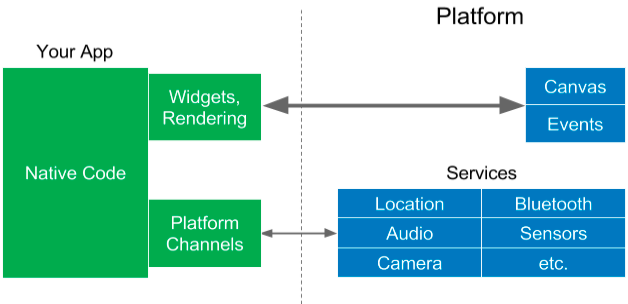
\includegraphics[width=\figureWidthModifier\linewidth]{img/stand-van-zaken/flutter-app-architecture.png}
    \caption{De architectuur van een Flutter applicatie \autocite{Leler2017}}
    \label{fig:flutter-app-architecture}
\end{figure}

Andere cross-platform frameworks zoals React Native, maken gebruik van een vertaler. In het geval van React Native is dit de JavaScript Bridge. De geschreven JavaScript code wordt door de JavaScript Bridge omgezet om de native platformen te kunnen aanspreken, zoals te zien op figuur \ref{fig:react-native-app-architecture}  \autocite{Kuitunen2019}

\begin{figure}[H]
    \centering
    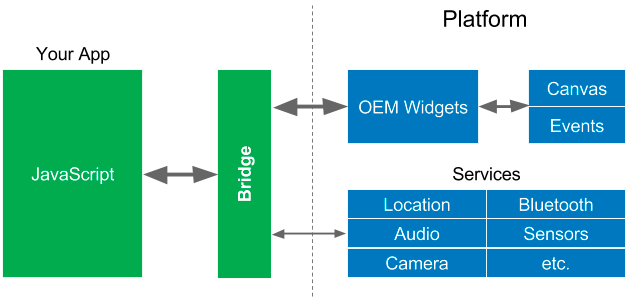
\includegraphics[width=\figureWidthModifier\linewidth]{img/stand-van-zaken/react-native-app-architecture.png}
    \caption{De architectuur van een React Native applicatie \autocite{Leler2017}}
    \label{fig:react-native-app-architecture}
\end{figure}

% TODO: supported platforms

\subsection{Flutter Web}
Flutter heeft hoofdzakelijk als platform mobiele apparaten, maar is zeker niet beperkt tot het maken van mobiele apps. Zo is Flutter Web in Flutter versie 1.9 beschikbaar als technical preview. Dit houdt in dat Flutter Web zelfs nog niet beschikbaar is in alfa of beta. Aangezien Flutter web zich nog in technical preview bevindt, wordt er aangeraden om Flutter web nog niet te gebruiken in productie. De werking van Flutter Web wordt in deze sectie verder besproken.
\newline
Opnieuw maakt de programmeertaal Dart het mogelijk om de Flutter code te compileren naar HTML, CSS en JavaScript.

Voor Flutter Web was het nodig dat de \verb|dart:ui| opnieuw geïmplementeerd werd. De \verb|dart:ui| library bestaat uit de laagst mogelijke services die Flutter gebruikt om toepassingen op te bouwen. Bijvoorbeeld klassen voor het aansturen van de invoer en grafische tekst. Hier werd de code dat beroep deed op de Skia Engine, herschreven naar doelgroepen als DOM en Canvas. De Skia Graphics Engine is een open-source grafische bibliotheek geschreven in C++. De \verb|dart:ui| library zorgt ervoor dat de Dart code gecompileerd wordt naar JavaScript en dus geschikt is voor web applicaties. Indien een widget niet omgezet kan worden in JavaScript, HTML en CSS, wordt het widget geschilderd op een canvas.
\newline
Met Flutter Web is het Flutter framework opnieuw een stap dichter naar een volledig cross-platform ontiwkkelingsomgeving.
Deze structuur wordt weergegeven in figuur \ref{fig:flutter-web-architecture}
\begin{figure}[H]
    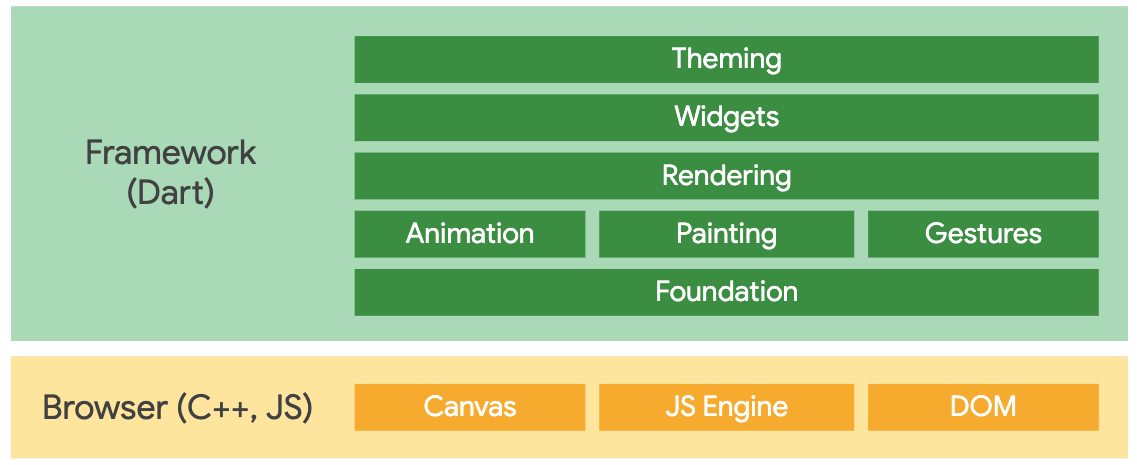
\includegraphics[width=\linewidth]{img/stand-van-zaken/flutter-web-architecture.png}
    \caption{De architectuur van Flutter Web \autocite{Flutter2019}}
    \label{fig:flutter-web-architecture}
\end{figure}


\subsection{Dart}
\label{ch:dart}
De taal die Flutter gebruikt is Dart. De populariteit van deze taal is de laatste tijd gestegen, mede dankzij de populariteit van Flutter. Met een groei van 532\% afgelopen jaar, kan Dart bekroond worden als de snelst groeiende taal \autocite{Chan2019}. 
Dit gedeelte is voornamelijk gebasseerd op een artikel van een Senior Software Engineer bij Google, Wm Leler \autocite{Leler2017a}.

De syntax van Dart is gelijkaardig aan die van Java, C\# en Javascript.
Een belangrijke troef van Dart is dat het zowel Ahead Of Time (AOT) als Just In Time (JIT) gecompileerd kan worden. Het feit dat Dart AOT gecompileerd kan worden heeft als gevolg dat een Flutter app in productie gebruik maakt van native prestaties. Dit zorgt voor een snelle en performante applicatie in productie.
De JIT compilatie lost de verwachtingen van elke ontwikkelaar in. De JIT zorgt ervoor dat wijzigingen tijdens het ontwikkelen van de applicatie quasi direct zichtbaar zijn op het apparaat. De JIT ondersteuning in Dart maakt het mogelijk dat Flutter over Hot Reloading beschikt. \autocite{Leler2017a}
\newline
Op dit moment is de laatste stabiele versie van Dart 2.6.0. Met nieuwe toevoegingen in versie 2.3.0 zoals de spread operator (...) wordt Dart frequent bijgewerkt met nieuwe features. De verwachtingen van de ontwikkelaars worden ingelost door periodiek feedback te vragen aan de community \autocite{Thomsen2019}.

\section{State en State Management}
In deze sectie wordt het concept state en de bijhorende State Management uitvoerig besproken. Dit hoofdstuk is losstaand van Flutter, maar gaat dieper in op de begrippen state en State Management. Dit onderdeel is een aanleiding naar de volgende sectie State Management in Flutter. Het is nodig om deze sectie te begrijpen om verder te gaan met dit onderzoek.

\subsection{State}
\label{ch:state}
De state van een applicatie is alles dat bijgehouden wordt in het geheugen terwijl de applicatie draait. \autocite{Coninck2019}
Een simpel voorbeeld van state is het volgende: één invoerveld voor voornaam, één invoerveld voor achternaam en één knop die niet klikbaar is, de state van deze knop kan beschouwd worden als een variabele \textit{klikbaar = onwaar}. Op dit moment is de knop niet klikbaar. Indien de invoervelden een geldige invoer ontvangen, wordt de state van de knop bijgewerkt: \textit{klikaar = waar}. Dit resulteert in een klikbare knop. De state van de knop is afhankelijk van de state van de invoervelden. Dit is een relatief simpel voorbeeld, maar wanneer een applicatie groeit wordt dit een zeer complex probleem. Bijvoorbeeld wanneer een state van een bericht afhankelijk is van een factor op een andere pagina. De state zal op verschillende schermen gedeeld moeten worden.
In de breedst mogelijke zin is de state van een applicatie alles wat in het geheugen bestaat wanneer de app wordt uitgevoerd. 

\subsection{Het begrip State Management}
De manier waarop de state van een applicatie wordt benaderd, wordt State Management genoemd. Er zijn reeds tal van State Management libraries, zoals Redux en MobX die deze benadering vereenvoudigen. Deze benaderingen worden verder besproken in sectie \ref{ch:redux} en \ref{ch:mobx}. De bedoeling van een benadering van State Management is om de state op een overzichtelijke manier te beheren en makkelijk uit te breiden.

\section{State Management in Flutter}
De vorige secties in verband met state en State Management zijn losstaand van Flutter. In deze sectie wordt bekeken hoe de state specifiek in een Flutter applicatie kan benaderd worden.

\subsection{Ephemeral State en App State}
De Flutter documentatie definieert twee soorten states: Ephemeral State (lokaal) en App State (globaal).
Ephemeral State is de lokale state, ook wel de UI state genoemd. Deze state wordt beheerd door één enkele widget, bijvoorbeeld de geselecteerde index bij een tabbalk. Andere widgets zullen zelden dit soort state van buitenaf nodig hebben. Bij Ephemeral State is het niet nodig om een bepaalde benadering van State Management toe te passen op een widget. In dit geval kan de Stateful widget zijn state aanpassen door zijn \verb|setState()| functie aan te roepen.
Om terug het voorbeeld van het invoerveld te hernemen: er wordt geluisterd wanneer er een karakter wordt getypt in het veld. Vervolgens wordt de state van het invoerveld bijgewerkt en hierna wordt \verb|setState()| opgeroepen zodat het widget opnieuw wordt opgebouwd met de bijgewerkte waarde.
\newline
De andere soort state volgens de Flutter documentatie \autocite{Developers2019} is App State, ook wel shared state genoemd. Deze soort state wordt door verschillende widgets van de applicatie gedeeld.
Een voorbeeld van dit soort state: een lijst van nieuws artikels, die respectievelijk gemarkeerd kunnen worden als gelezen en niet-gelezen. Wanneer een artikel gemarkeerd is aan gelezen moet deze verwijderd worden van de lijst. 
\newline

Over het algemeen is er geen duidelijke regel wanneer Ephemeral State of App State gebruikt moet worden. Dit is volledige afhankelijk van de complexiteit van de applicatie en de persoonlijke voorkeur van de ontwikkelaar.
Wanneer een applicatie nood heeft aan de nodige complexiteit wordt er aangeraden om over te schakelen naar App State \ref{fig:ephemeral-vs-app-state-flutter}. Theoretisch is het mogelijk om een volledige applicatie te ontwikkelen met State en setState(), maar dit wordt afgeraden \autocite{Developers2019}.
\begin{figure}[H]
    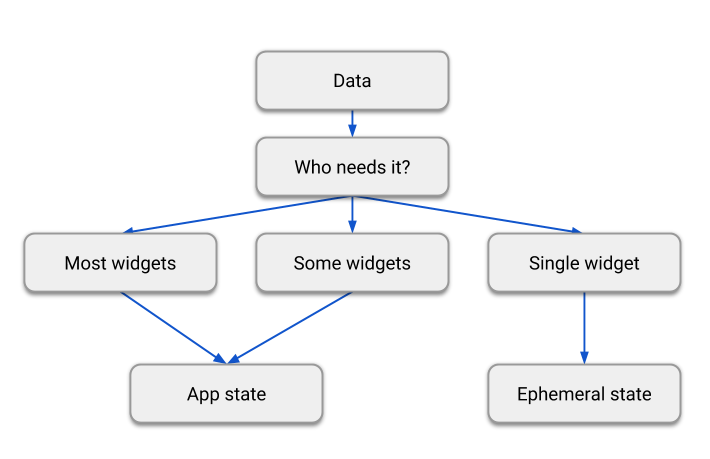
\includegraphics[width=\linewidth]{img/stand-van-zaken/ephemeral-vs-app-state-flutter.png}
    \caption{Ephemeral- vs App state in Flutter \autocite{Developers2019}}
    \label{fig:ephemeral-vs-app-state-flutter}
\end{figure}

Dit resulteert in het ontstaan van verschillende State Management benaderingen. Tal van benaderingen van State Management worden beschikbaar gesteld door middel van libraries. Deze State Mangement libraries zorgen dat het beheren van state in een applicatie versimpeld wordt.
Het doel van een State Management is om het leven van de ontwikkelaar eenvoudiger te
maken door state makkelijker beheersbaar te maken. Verder wordt de UI gescheiden van
de business logica, waardoor deze logica makkelijker getest kan worden.

In volgende sectie worden de verschillende benaderingen van State Management in Flutter besproken.
De verschillende benaderingen die besproken worden zijn: 
\begin{itemize}
    \item ScopedModel
    \item Provider
    \item BLoC met RxDart
    \item Redux
    \item MobX
\end{itemize}

\subsection{ScopedModel}
Wanneer er nood is aan een relatief simpele benadering van State Management in een Flutter applicatie is ScopedModel een geschikte kandidaat \autocite{Boelens2019}. ScopedModel geeft een Model door naar onderliggende widgets, \textit{van vader naar kinderen}. ScopedModel is opgebouwd rond drie belangrijke concepten, een Model, een ScopedModel en een ScopedModelDescendant die te zien zijn op figuur \ref{fig:scopedmodel}. 

\begin{figure}[H]
    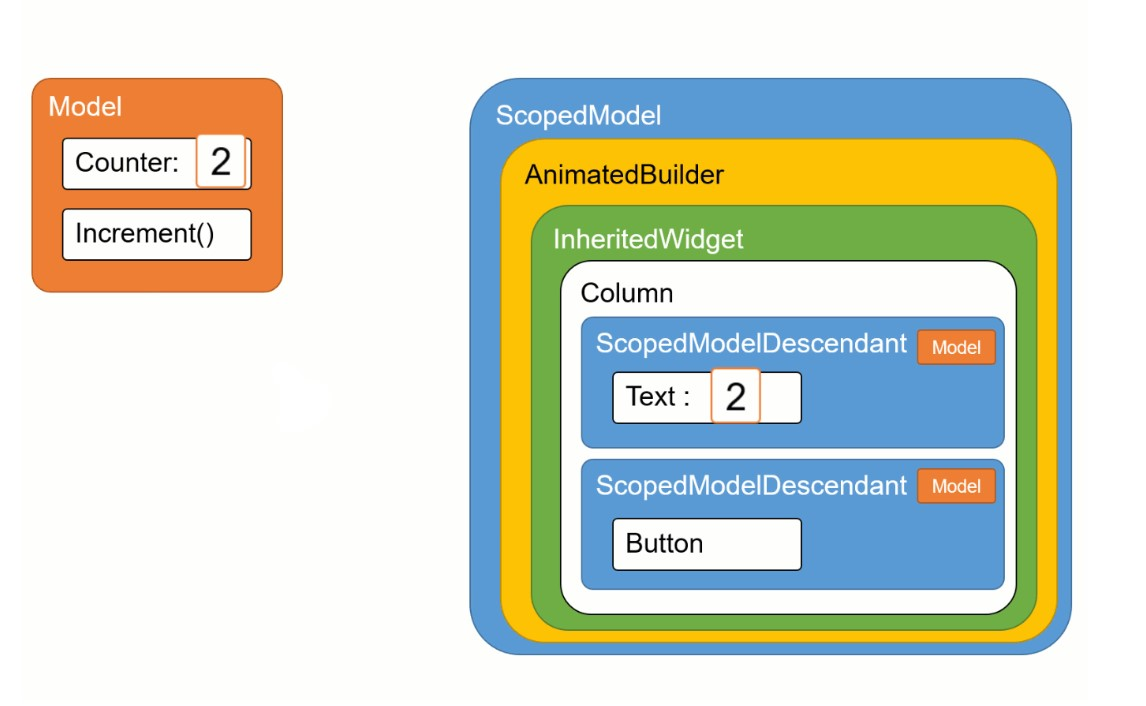
\includegraphics[width=\linewidth]{img/stand-van-zaken/scopedmodel.jpg}
    \caption{De drie concepten bij ScopedModel \autocite{Boelens2019}}
    \label{fig:scopedmodel}
\end{figure}
Als eerst wordt een klasse gedefinieerd die de 
data en business logica zal bijhouden. Deze klasse heeft als kenmerk dat er geluisterd kan worden naar deze klasse. Als er in de Model klasse een wijziging aangebracht wordt laat de klasse de wijziging aan zijn kinderen weten via \verb|notifyListeners()|.
\newline
De ScopedModel widget maakt het mogelijk om een Model mee te geven, dit zorgt ervoor dat al de kinderen van deze ScopedModel toegang hebben tot het meegegeven Model. Een kind van een ScopedModel kan het Model oproepen met \verb|ScopedModel.of<Model>(context)|.

Als laatste gebruikt ScopedModel een ScopedModelDescendant, dit is een speciale widget. Deze widget reageert automatisch op wijzigingen in het Model. Als \verb|notifyListeners()| wordt opgeroepen wordt deze widget .
ScopedModelDescendant heeft een verplichte \verb|builder| functie. Het type van Model waar de widget naar luistert wordt gedefinieerd tussen \verb|< >|
\begin{minted}{dart}
ScopedModelDescendant<CounterModel>(
    builder: (context, child, model) {
        return Text(model.counter);
    },
);
\end{minted}
Hier wordt geluisterd naar een wijziging in een \verb|CounterModel|. Wanneer deze wijzigt, met andere woorden \verb|notifyListeners()| wordt opgeroepen in het model, wordt de \verb|builder| functie aangeroepen. De waarde van de counter wordt op het scherm getoond. Nu is het mogelijk om op een ander scherm de counter te verhogen en wordt de tekst automatisch opnieuw opgebouwd. Er kan ook gebruikt gemaakt worden van \verb|ScopedModel.of<CounterModel>(context)| om het model in eender welke widget op te roepen. 

Indien nood is aan meerdere modellen, kunnen de ScopedModelDescendant widgets genest worden of opnieuw via de static methode \verb|ScopedModel.of| opgeroepen worden.

\subsection{Provider}
\subsection*{Principes}
Een nieuwkomer in het Flutter framework wordt aangeraden om de Provider package te hanteren. Provider zorgt voor een snelle benadering van State Management zonder al te veel complexiteit. Provider biedt een oplossing voor State Management en Dependency Injection.
De Provider package maakt het mogelijk om data beschikbaar te maken voor widgets die het nodig hebben. Op voorwaarde dat de Provider widget als voorouder wordt geplaatst in de widget tree.

De volgende code is gegeven:
\begin{minted}{dart}
Provider<CounterModel>(
    builder: (BuildContext context) => CounterModel(),
    dispose: (BuildContext context, CounterModel counterModel) {
        counterModel.dispose(),
    },
    child: Container(),
);
\end{minted}

Hier wordt een CounterModel eenmalig aangemaakt. Vervolgens wordt met de \verb|dispose()| methode meegegeven wat er moet gebeuren als het Provider widget wordt verwijderd uit de widget tree. Nu is het mogelijk om in de kinderen van de Provider widget het CounterModel op te vragen via \verb|final counterModel = Provider.of<CounterModel>(context)|.
Bijvoorbeeld in de Container die wordt meegegeven aan het \verb|child| property.

De functie \verb|Provider.of<T>(context, listen: false)| heeft zoals gegeven een \verb|listen| optie. Als \verb|false| wordt meegegeven wordt de widget niet herbouwd bij een wijziging. Bij sommige omstandigheden kan dit van toepassing zijn zodat onnodige rebuilds vermeden worden. Aangezien de Provider widget de totale controle heeft over het moment waarop de waarde wordt opgevraagd is er een zekerheid dat de waarde niet tweemaal wordt opgevraagd. Met andere woorden de waarde wordt niet tweemaal geïnstantieerd.

\subsection*{Werking}
De werking van de Provider package beperkt zich niet alleen tot het voorzien (provide) van een waarde, maar heeft zoals eerder vermeld, ook een meldfunctionaliteit (notify).
In de documentatie van de package zijn tal van Provider variaties beschikbaar: \verb|ListenableProvider|, \verb|ChangeNotifierProvider|, \verb|ChangeNotifierProxyProvider|, \verb|ValueListenableProvider|, \verb|StreamProvider| en \verb|FutureProvider|. Als laatste is, zoals reeds vermeld, een \verb|Consumer| widget beschikbaar.
De \verb|ListenableProvider| is een specifieke implementatie voor het \verb|Listenable| object. De \verb|ListenableProvider| luistert naar data en vraagt aan de afhankelijke widgets om opnieuw te renderen wanneer de listener wordt opgeroepen. In de praktijk wordt de \verb|ListenableProvider| niet direct gebruikt, maar wel indirect. De \verb|ChangeNotifierProvider| is een specificatie van de \verb|ListenableProvider| voor \verb|ChangeNotifier|; Hier wordt de \verb|ChangeNotfier.dispose| automatisch opgeroepen wanneer nodig.

Recentelijk is de \verb|MultiProvider| toegevoegd. Deze widget biedt een oplossing tegen het nesten van Provider widgets. Stel er is nood aan twee modellen doorheen een applicatie. Het eerste model wordt meegegeven aan de Provider widget. Het tweede model wordt opnieuw meegegeven aan een Provider widget. Dit resulteert in volgende code:
 \begin{minted}{dart}
 Provider<CounterModel>(
    builder: (BuildContext context) => CounterModal(),
    dispose: (BuildContext context, CounterModel counterModel) {
        counterModel.dispose(),
    },
    child: Provider<PreferenceModel>(
        builder: (BuildContext context) => PreferenceModel(),
        dispose: (BuildContext context, PreferenceModel preferenceModel) {
            preferenceModel.dispose(),
        },
    ),
);
\end{minted}
Dit resulteert in het nesten van Provider widgets, dit probleem wordt opgelost door de \verb|MultiProvider|. Volgende code is idem aan bovenstaande, maar is overzichtelijker en stimuleert de leesbaarheid van de code.
 \begin{minted}{dart}
MultiProvider(
    providers: [
        Provider<CounterModel>(
            builder: (BuildContext context) => CounterModel(),
            dispose: (BuildContext context, CounterModel counterModel) {
                counterModel.dispose(),
            },
        ),
        Provider<PreferenceModel>(
            builder: (BuildContext context) => PreferenceModel(),
            dispose: (BuildContext context, PreferenceModel preferenceModel) {
                preferenceModel.dispose(),
            },
        ),
    ],
    child: Container(),
);

\end{minted}

De Provider package biedt twee manieren aan om op de hoogte te worden gebracht.
\newline
De eerste manier is via de static methode \verb|Provider.of(context)| met een optionele \verb|listen| property, standaard op \verb|true|.
Wanneer een widget zichzelf registreert als een dependency van de Provider InheritedWidget, zal het telkens opnieuw opgebouwd worden wanneer de data wijzigt. Een InheritedWidget is een klasse voor widgets die informatie efficiënt door de boom heen wil verspreiden.
 Meer bepaald wanneer \verb|notifyListeners()| wordt opgeroepen. Of wanneer een \verb|StreamProvider| zijn stream nieuwe data uitzendt of wanneer een FutureProvider zijn future is voltooid. Een Future in Dart wordt gebruikt om een potentiële waarde of fout weer te geven die ergens in de toekomst beschikbaar zal zijn, met andere woorden een asynchrone operatie. Een future is te vergelijkbaar met een Promise in JavaScript.

De tweede manier is om gebruik te maken van de \verb|Consumer| widget. Deze widget is een hulp widget die in de achtergrond de \verb|Provider.of(context)| gebruikt. De werking van de \verb|Consumer| is gelijkaardig aan die van de bovenstaande. 

De \verb|Provider| package is gelijkaardig aan de \verb|ScopedModel| benadering. Waar \verb|Provider| een volledige oplossing biedt voor dependency injection, probeert \verb|ScopedModel| zich op te stellen als een architecturale oplossing.

\subsection{BLoC met RxDart}
\subsection*{Business Logic Component}
Het BLoC patroon dat staat als afkorting voor Business Logic Component. Het BLoC werd oorspronkelijk aangeboden als oplossing voor het delen van dezelfde business logica tussen Flutter en AngularDart. AngularDart is een open-source project gebouwd bovenop het Dart Web Platform, het wordt veelal gebruikt voor het ontwikkelen van web applicaties in Dart. Hedendaags wordt BLoC door Google aangeraden als een superieure State Management techniek. Het BLoC pattern maakt gebruik van Streams die beschikbaar zijn in Dart, maar vaak wordt beroep gedaan op een gebruiksvriendelijkere library namelijk ReactiveX, zie \ref{ch:reactivex}. De ReactiveX library is een laag bovenop de Streams.
\newline
De ReactiveX (rX) library is in Dart beschikbaar onder de naam RxDart.

\subsection*{Streams}
Om het BLoC patroon volledig te begrijpen moet het concept Streams uitgelegd worden.
Een stream kan gevisualiseerd worden als een pipe met twee uiteinden, waarvan slechts
één uiteinde gebruikt kan worden om iets in de pipe te plaatsen en het andere dient als de uitgang. Wanneer data in de pipe
geplaatst wordt, stroomt het door de pipe naar het andere uiteinde. \autocite{Boelens2018}

\begin{figure}[H]
    \centering
    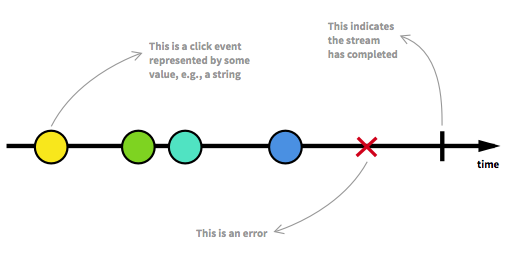
\includegraphics[width=\figureWidthModifier\linewidth]{img/stand-van-zaken/stream-pipeline.png}
    \caption{Voorbeeld van een Stream pipeline \autocite{Staltz2019}} 
    \label{fig:stream-pipeline}
\end{figure}

In Flutter kan het concept van Streams gemakkelijk gebruikt worden. De effectieve pipe wordt voorgesteld als een Stream. Deze \verb|Stream| klasse op zich maakt het niet mogelijk om deze pipe te beheren.
Daarvoor wordt een \verb|StreamController| gebruikt. Om toegang te krijgen tot de invoer van een pipe, wordt beroep gedaan op een \verb|StreamSink|. Deze wordt door de \verb|StreamController| beschikbaar gesteld via de \verb|sink| property.

Zowel primitieve data types als objecten en errors kunnen voorgesteld worden als een stream. Een stream heeft geen beperkingen op vlak van soorten data types.

Om wijzigingen van een stream in acht te nemen kan er geluisterd worden naar een stream, dit resulteert in een \verb|StreamSubscription|. Deze \verb|StreamSubscription| is beschikbaar via de \verb|stream| property van de StreamController. Deze geeft meldingen wanneer er wijzigingen gebeuren in de stream, bijvoorbeeld wanneer een nieuwe waarde wordt toegevoegd op deze stream.

Met andere woorden heeft een pipe één toegang, de sink en één uitgang, de stream.

Als er minstens één actieve luisteraar van een stream is, start de stream met het genereren van events die de \verb|StreamSubscription| verwittigt wanneer een wijziging zich voordoet. Deze events worden opgeroepen bij volgende scenario's: er is een error in de stream, de stream wordt afgesloten of er is nieuwe data in de stream.

De \verb|StreamTransformer| zorgt ervoor dat de data in de stream gemanipuleerd kan worden. Onder deze manipulaties worden volgende verstaan: filteren, hergroeperen, aanpassen, data in andere streams injecteren...
Een voorbeeld van een StreamTransformer manipulatie op een Stream:
 \begin{minted}{dart}
final streamTransformer = StreamTransformer<num, num>.fromHandlers(
    handleData: (num data, EventSink sink) {
        // De data wordt vermenigvuldigd met 2
        sink.add(data * 2);
    }, 
    handleError: (Object error, StackTrace stacktrace, EventSink sink) {
        // Voeg de error toe aan de stream via de sink
        sink.addError('Er ging iets fout: $error');
    }, 
    handleDone: (EventSink sink) => sink.close(),
);
\end{minted}

Bij streams zijn er twee soorten types: single-subscription- en broadcast streams. Bij een single-subscription stream kan er slechts één luisteraar geabonneerd zijn, zelfs wanneer de subscription geannuleerd wordt. Indien er een tweede maal geluisterd wordt naar een single-subscription stream wordt een gepaste error gegeven: \verb| Stream has already been listened to|.

Bij een broadcast stream kunnen er meerdere luisteraars zijn. Het is mogelijk om op elk moment een luisteraar aan een broadcast stream toe te voegen. De nieuwe luisteraar ontvangt de gebeurtenissen vanaf het moment dat deze naar de stream begint te luisteren.

De implementatie van de stream library wordt standaard meegeleverd in de Software Development Kit (SDK) van Flutter. Om een stream te visualiseren in een widget wordt de StreamBuilder widget gebruikt. Een StreamBuilder is geïmplementeerd als een StatefulWidget die opnieuw wordt opgebouwd wanneer nieuwe events gestreamd worden.
Een voorbeeld van zo'n StreamBuilder:
\begin{minted}{dart}
StreamBuilder<Counter>(
    stream: counterStream,
    initialData: 0,
    builder: (context, snapshot) {
        if (snapshot.hasData){
            return Text(snapshot.data);
        }
        return CircularSpinner();
    },
);
\end{minted}
De initiële data wordt ingesteld op 0 wanneer de \verb|counterStream| nog geen data bevat. Dit dat de StreamBuilder widget bij de initiële render 0 zal gebruiken als data. De \verb|builder| functie zorgt ervoor dat de StreamBuilder weet welke widget opgebouwd moet worden wanneer de \verb|StreamBuilder| nieuwe data ontvangt via de \verb|stream| property.

In volgende sectie wordt het rxDart package besproken, deze package breidt de functionaliteit van de originele Dart Streams uit om te voldoen aan de ReactiveX standaarden.

\subsection*{ReactiveX in Dart}
\label{ch:reactivex}
De ReactiveX library is een library die de functionaliteiten van streams in een programmeertaal uitbreidt. Zo is ReactiveX beschikbaar in JavaScript onder de naam RxJS, maar relevanter voor dit onderzoek, in Dart: de RxDart library.


Zoals reeds vermeld is de RxDart package een implementatie van de ReactiveX API in Dart. Zowel Dart Streams als RxDart worden gebruikt om streams te maken en beheren, maar beide ontwikkelaars gebruiken een andere terminologie.
Een Stream in Dart wordt voorgesteld als een \verb|Observable| in RxDart. Een StreamController is een \verb|Subject| in RxDart, zie tabel \ref{table:terminologie-rxdart-dart}.

\begin{table}[H]
    \centering
    \begin{tabular}{ll}
        \textbf{Dart}    & \textbf{RxDart} \\ \hline
        Stream           & Observable      \\
        StreamController & Subject         \\
        &                
    \end{tabular}
    \caption{Verschillende Stream terminologie in Dart en RxDart \autocite{Boelens2018}}
    \label{table:terminologie-rxdart-dart}
\end{table}

RxDart biedt drie variaties van de StreamController.
\newline 
De PublishSubject, geïllustreerd op figuur \ref{fig:rxdart-publishsubject}, is een normale broadcast StreamController. In dit diagram wordt enkel data van de stream gestuurd, nadat er naar de stream geluisterd (geabonneerd) wordt.
Merk op dat deze variaties een Observable terug geven in plaats van een Stream zie tabel \ref{table:terminologie-rxdart-dart}.


\begin{figure}[H]
    \centering
    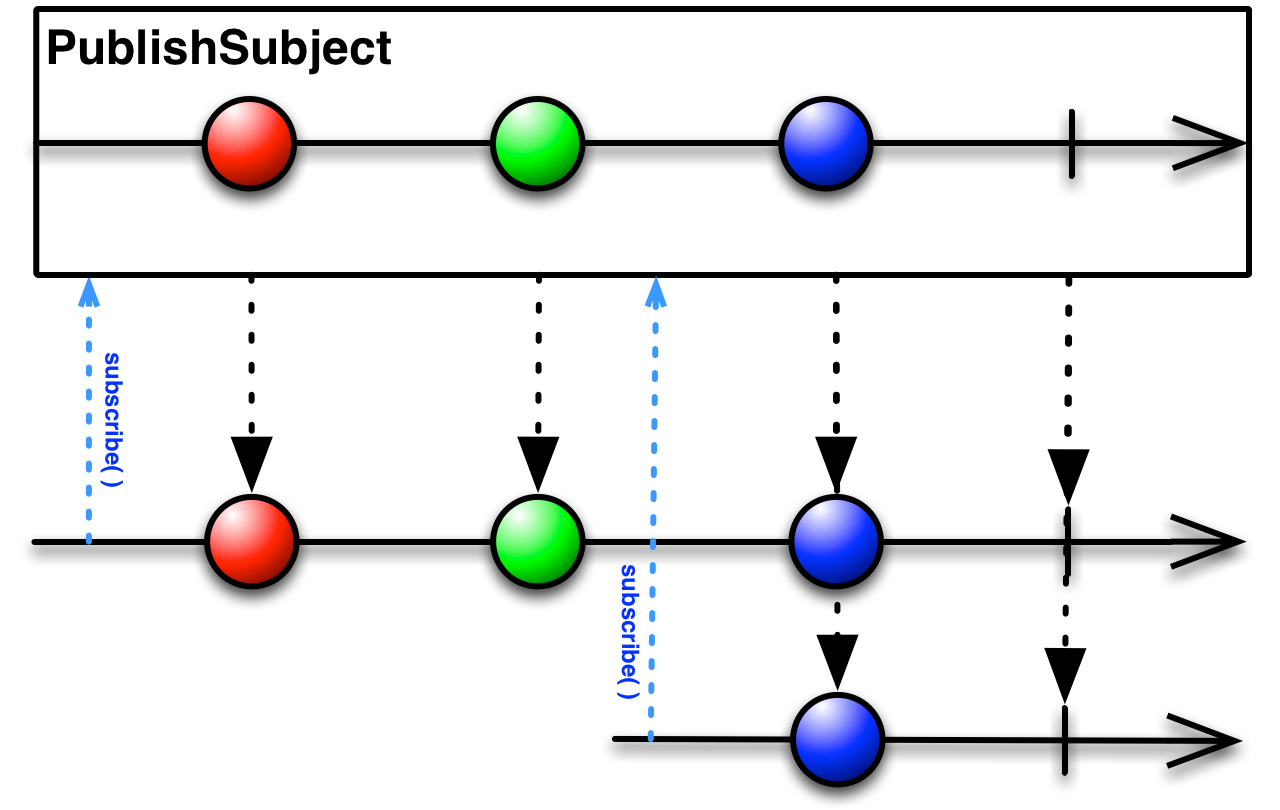
\includegraphics[width=\figureWidthModifier\linewidth]{img/stand-van-zaken/rxdart-publishsubject.png}
    \caption{Marble diagram van PublishSubject uit de ReactiveX library \autocite{Boelens2018}}
    \label{fig:rxdart-publishsubject}
\end{figure}

De tweede variatie is een BehaviorSubject, ook dit is een broadcast StreamController. Hier wordt de laatst toegevoegde data van de stream uitgezonden. Ook al was de luisteraar nog niet geabonneerd op het moment dat de laatste data werd uitgezonden. Zie figuur \ref{fig:rxdart-behaviorsubject}. 

\begin{figure}[H]
    \centering
    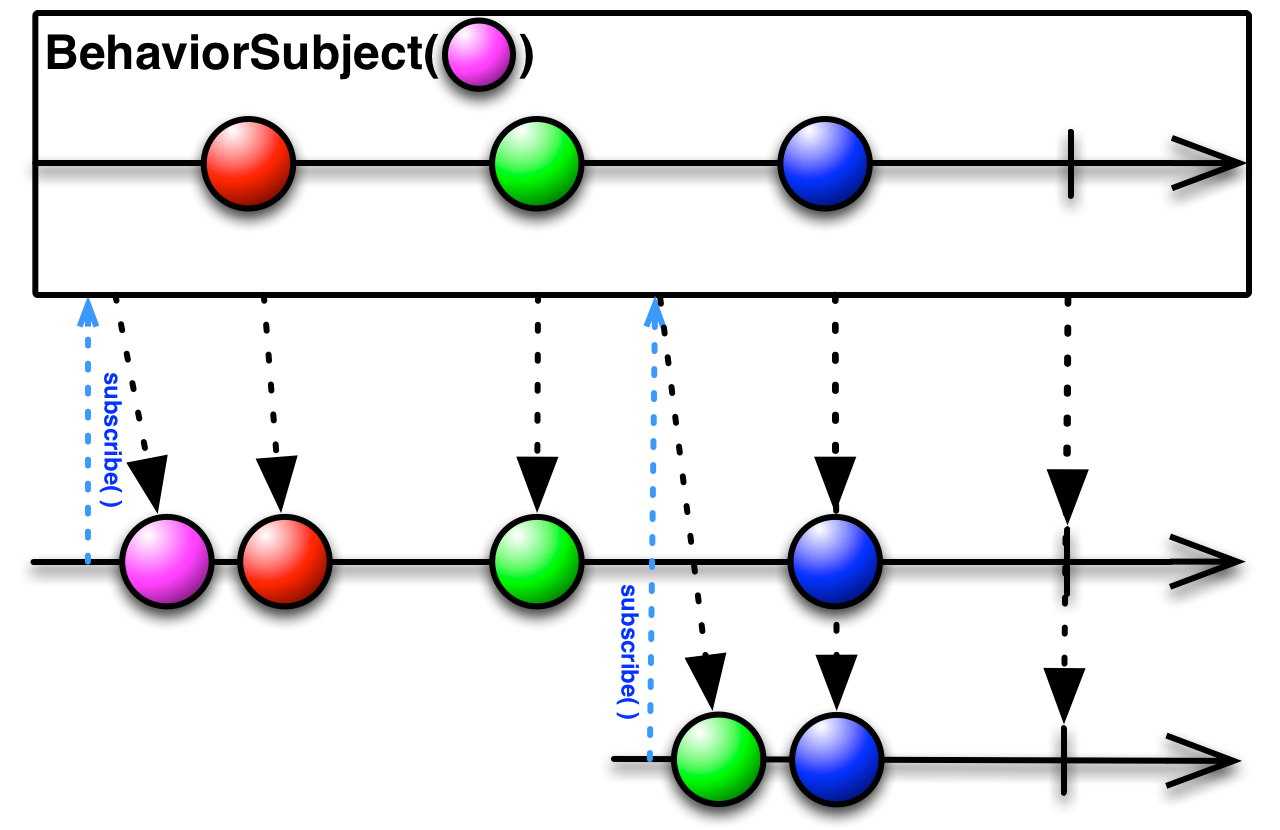
\includegraphics[width=\figureWidthModifier\linewidth]{img/stand-van-zaken/rxdart-behaviorsubject.png}
    \caption{Marble diagram van BehaviorSubject uit de ReactiveX library \autocite{Boelens2018}}
    \label{fig:rxdart-behaviorsubject}
\end{figure}

Als derde variatie is er de ReplaySubject. Dit is een broadcast StreamController die alle events uitzendt naar zijn luisteraars die reeds zijn voorgekomen sinds het begin van de stream zijn levencyclus. Zie figuur \ref{fig:rxdart-replaysubject}.

\begin{figure}[H]
    \centering
    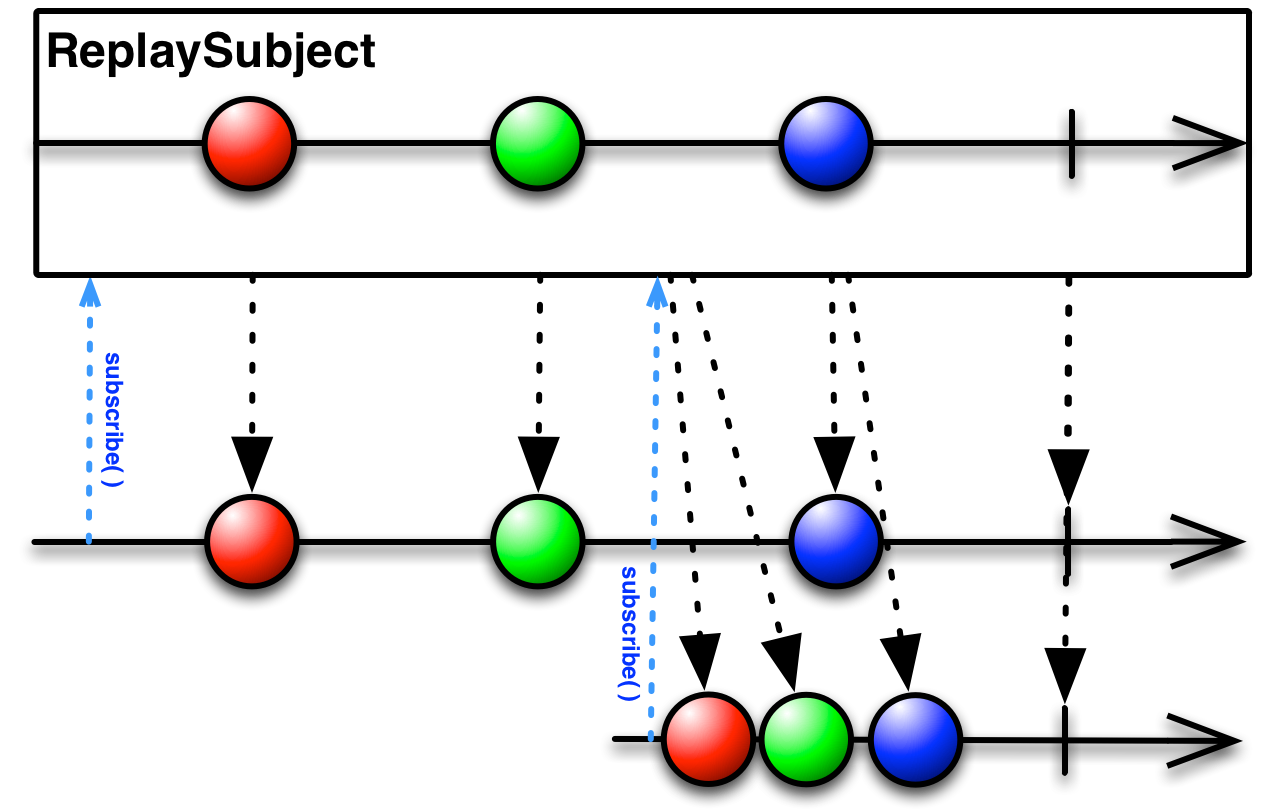
\includegraphics[width=\figureWidthModifier\linewidth]{img/stand-van-zaken/rxdart-replaysubject.png}
    \caption{Marble diagram van ReplaySubject uit de ReactiveX library\autocite{Boelens2018}}
    \label{fig:rxdart-replaysubject}
\end{figure}

\subsection*{Het leven van het BLoC patroon}
De toepassing van het BLoC patroon is dat alle business logica zoveel mogelijk wordt losgekoppeld van de presentatie laag. Deze business logica kan opgesplitst worden in verschillende Business Logic Components (BLoCs). 
\newline
Enkele voordelen zijn: 
\begin{itemize}
    \item Er kunnen aanpassingen gedaan worden in de business logica zonder dat de presentatielaag aangepast wordt.
    \item De business logica kan makkelijk hergebruikt worden doorheen het project, zo ook voor externe projecten die beroep doen op dezelfde business logica.
    \item Het is eenvoudiger om de business logica te testen.
\end{itemize}
Zie structuur BLoC patroon op figuur \ref{fig:bloc-pattern}.

\begin{figure}[H]
    \centering
    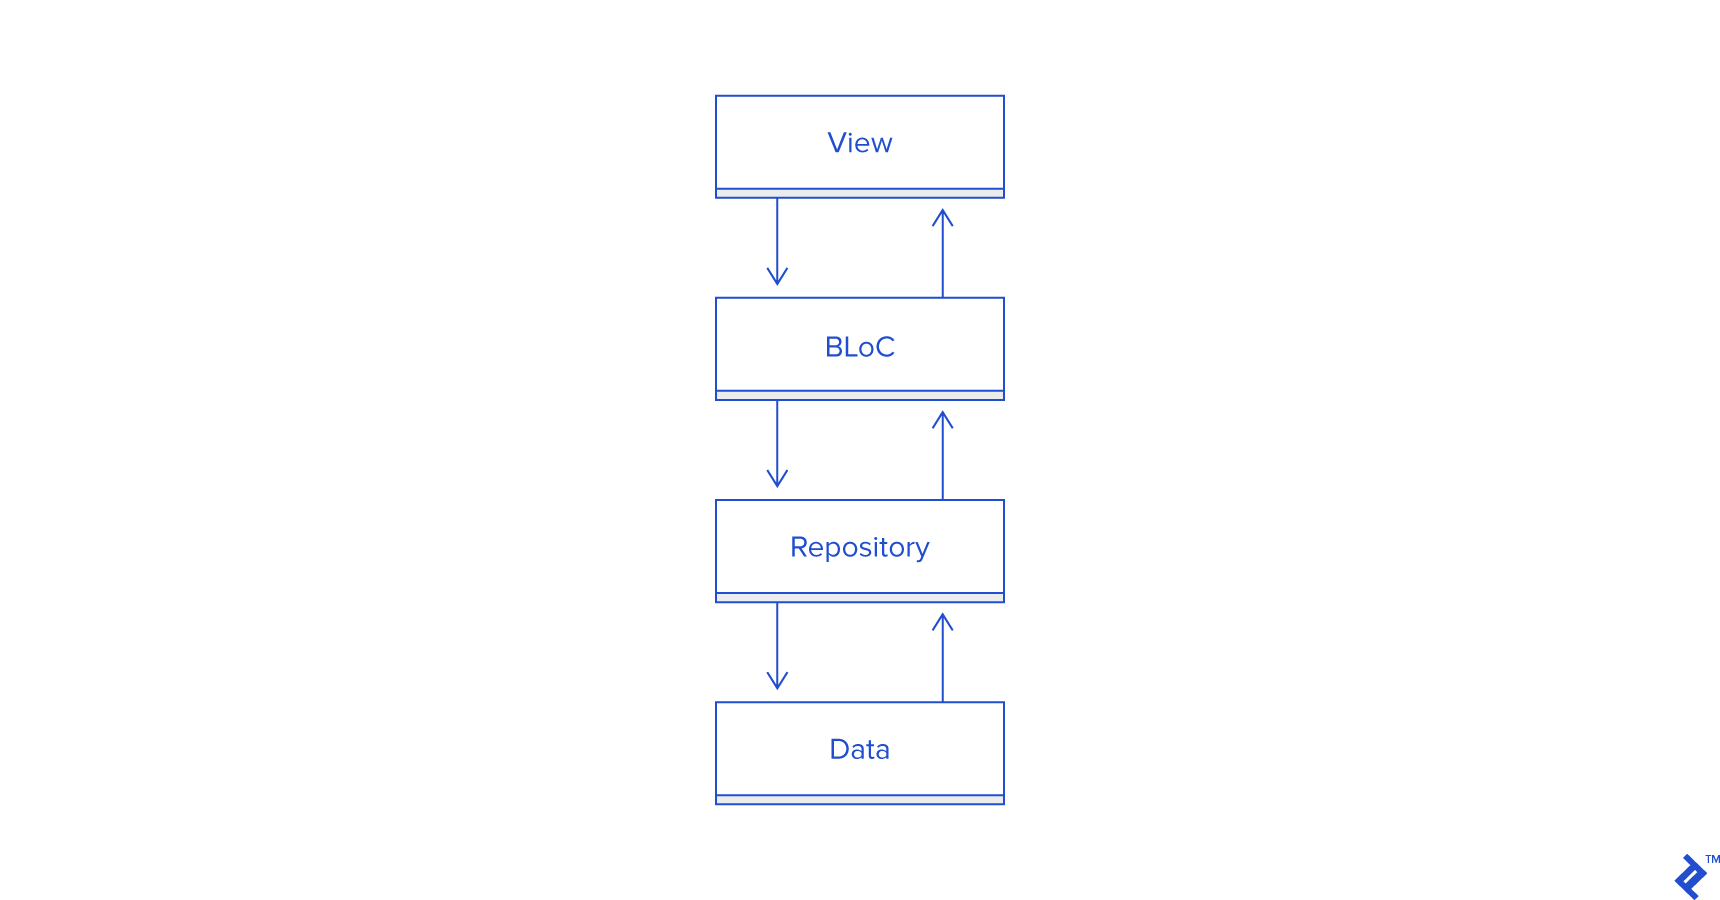
\includegraphics[width=0.9\linewidth]{img/stand-van-zaken/bloc-pattern.png}
    \caption{Concept van het BLoC patroon \autocite{Perutovic2018}}
    \label{fig:bloc-pattern}
\end{figure}

Bij het BLoC patroon zenden widgets events naar de BLoC via sinks en luisteren ze naar de streams van de BLoC.
Anders gezegd: de input van het BLoC de sink is en de output van het BLoC de stream. Een widget die luistert naar een stream wordt bijgewerkt wanneer er nieuwe data is. Bij deze benadering van State Management moet de widget in de presentatie geen kennis hebben van de business logic zoals te zien op figuur \ref{fig:bloc-pattern-streams-sinks}. \\


\begin{figure}[H]
    \centering
    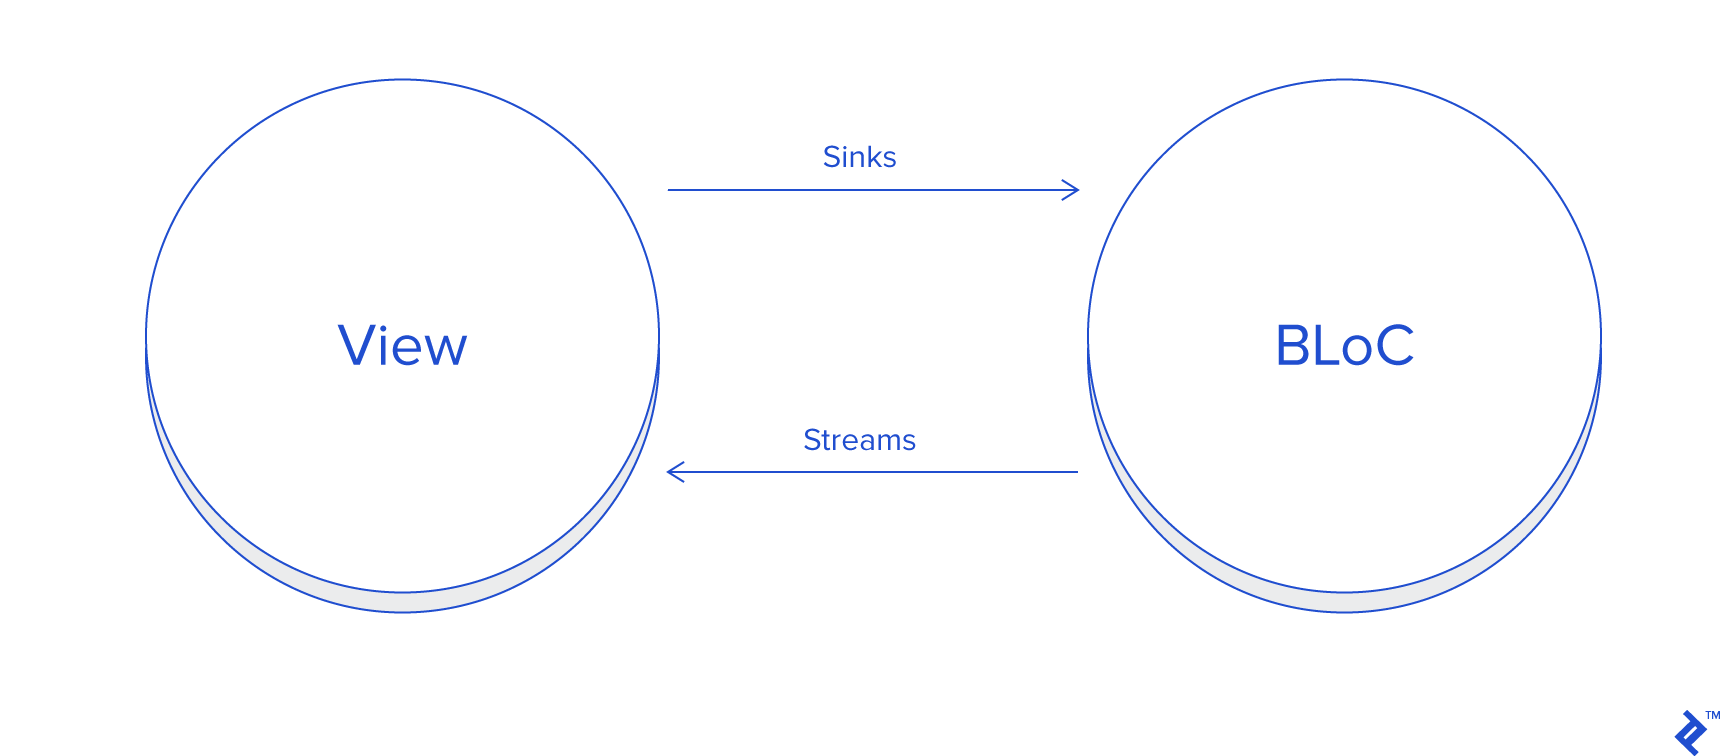
\includegraphics[width=\figureWidthModifier\linewidth]{img/stand-van-zaken/bloc-pattern-streams-sinks.png}
    \caption{Streams en Sinks tussen de presentatie en business logica \autocite{Perutovic2018}}
    \label{fig:bloc-pattern-streams-sinks}
\end{figure}

Er zijn verschillende manieren om de BLoC beschikbaar te stellen aan de widgets. 
Als eerste via een globale singleton. Dit wordt niet aangeraden aangezien er geen class destructor is in Dart, met andere woorden: mogelijkheid op memory leaks. Dart is een garbage-collected taal dit wil zeggen dat elk object, waar er geen verwijzing naar is, wordt door het runtime-systeem vrijgegeven. 
Een tweede mogelijkheid is om een lokale instantie te maken van de BLoC. Dit is een werkbare oplossing onder sommige omstandigheden. Merk hierbij op dat deze lokale instantie gemaakt wordt in een StatefulWidget, zodat de subscriptions op de streams in de \verb|dispose()| beëindigd kunnen worden.
De laatste en ook meest voorkomende manier is om de BLoC mee te geven aan een voorouder widget, die een implementatie is van een InheritedWidget of een StatefulWidget. Deze widget zorgt ervoor dat de BLoC ter beschikking gesteld wordt voor al zijn nakomelingen. Hiervoor wordt gebruikt gemaakt van een \verb|InheritedWidget|. Deze widget zorgt ervoor dat de nakomelingen in deze widget tree toegang hebben tot de BLoC.

\subsection{Redux}
\label{ch:redux}
\subsection*{Principes}
Redux is een gekende library voor het beheren van state. De library is vooral gekend bij JavaScript ontwikkelaars en wordt vaak gebruikd in Angular of React applicaties. Angular en React zijn beiden JavaScript frameworks voor het ontwikkelen van web applicaties. Echter is de library ook bruikbaar voor Flutter applicaties, aangezien de concepten dezelfde zijn. De package is beschikbaar in de package manager van Dart (pub.dev) onder de naam \verb|flutter_redux|.

Een toelichting over een paar begrippen die voorkomen in Redux.
Actions beschrijven alleen maar wat er gebeurd is. Elke action beschikt over een reducer, die de state aanpast.

Een Reducer is een synchrone functie die enige verwerking uitvoert op basis van de combinatie action - state. De manipulatie van de state leidt kan tot een nieuwe state in de Store. De Reducer is de enige die de state mag veranderen. Op deze manier zit de business logica alleen verwerkt in de Reducer. 

Een Middleware is een functie, meestal gericht op het uitvoeren van asynchrone taken, gebasseerd op een Action. Een Middleware maakt gebruik van State maar wijzigt deze niet. Een voorbeeld van een Middleware kan een logger functie zijn. Een ontwikkelaar kan ervoor zorgen dat elke action gelogd wordt, dit kan met behulp van een Middleware.

Redux bestaat uit een paar verschillende principes: er wordt gebruik gemaakt van een unidirectionele data flow. De store houdt maar één state bij en heeft maar één aanspreekpunt, namelijk via \verb|dispatch|. De \verb|dispatch| accepteert alleen maar \verb|actions| als argument.

Volgens de officiële documentatie van Redux \autocite{Redux2019} is het een good practice om per applicatie slechts een enkele Store te hebben. Indien het toch gewenst is om de data handling te scheiden wordt aangeraden om \verb|reducer composition| toe te passen in plaats van meerdere stores te maken.

\subsection{Werking}
Over het algemeen is de werking van Redux samen te vatten zoals op de figuur \ref{fig:redux-working}. Een applicatie bevat state. Deze state wordt aan een gebruiker getoond in de presentatielaag. Wanneer de presentatielaag een wijziging teweeg brengt, bijvoorbeeld door een klik op een knop, wordt een Action opgeroepen. De Action wordt ontvangen door een Reducer. Deze reducer werkt de Store bij waar de State van de applicatie wordt bijgehouden. Merk op dat deze Action door een Middleware kan passeren vooraleer deze wordt afgehandeld door een Reducer.

\begin{figure}[H]
    \centering
    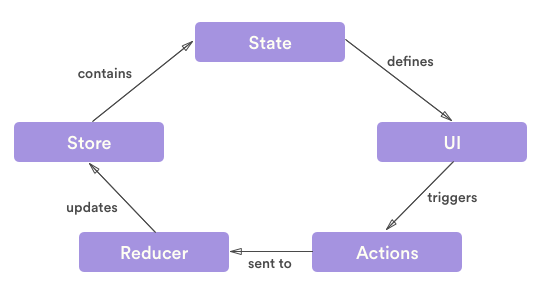
\includegraphics[width=\linewidth]{img/stand-van-zaken/redux-working.png}
    \caption{Werking van Redux \autocite{Tahir2018}}
    \label{fig:redux-working}
\end{figure}

Aangezien de manier in Redux voor vele ontwikkelaars een wijziging in de gedachtegang veresit, wordt een situatie in Redux geschetst waarbij elke stap uitvoerig wordt besproken.
Stel een applicatie toont een pagina met één knop. De applicatie bevindt zich in een initiële state. Dit wordt voorgesteld in figuur \ref{fig:redux-working-detailed-1}.

\begin{figure}[H]
    \centering
    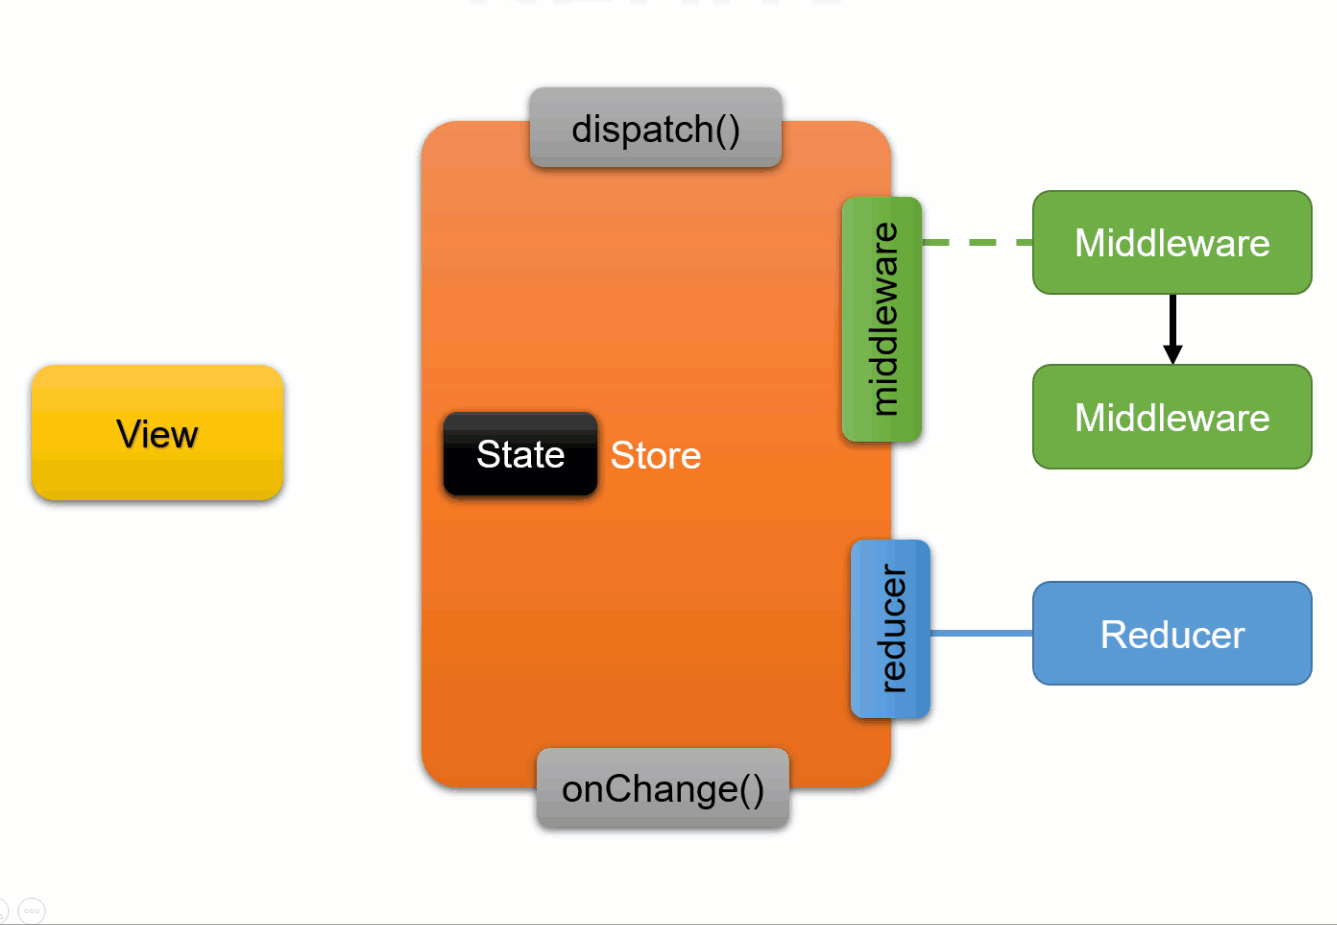
\includegraphics[width=\figureWidthModifier\linewidth]{img/stand-van-zaken/redux-working-detailed-1.png}
    \caption{Initiële situatie in een Redux State Management benadering \autocite{Boelens2019}}
    \label{fig:redux-working-detailed-1}
\end{figure}

Wanneer op een knop wordt geklikt, wordt een Action aangemaakt en uitgezonden naar de Store, dit is te zien op figuur \ref{fig:redux-working-detailed-2}. Dit uitzenden gebeurt via de \verb|store.dispatch(action)|. Indien voor de Action Middleware geconfigureerd is, wordt de Middleware sequentieel opgeroepen. Merk op dat tijdens de verwerking van deze Middleware een nieuwe Action kan verzonden worden naar de Store.

\begin{figure}[H]
    \centering
    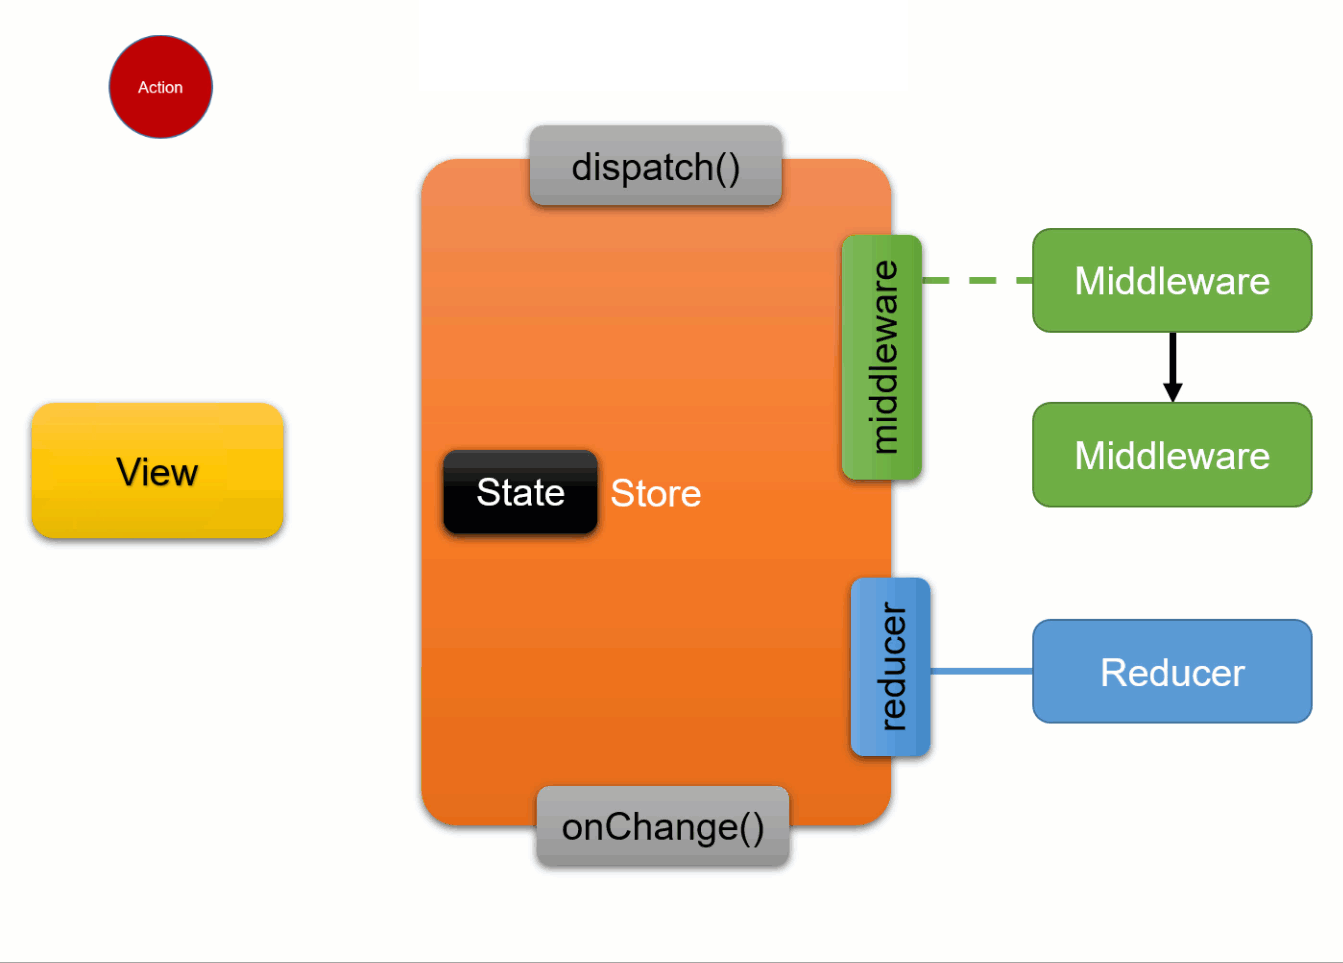
\includegraphics[width=\figureWidthModifier\linewidth]{img/stand-van-zaken/redux-working-detailed-2.png}
    \caption{een Action wordt gemaakt en verzonden naar de Store \autocite{Boelens2019}}
    \label{fig:redux-working-detailed-2}
\end{figure}

Vervolgens worden de Action en de nieuwe State doorgestuurd naar de Reducer, te zien op figuur \ref{fig:redux-working-detailed-3}. De Reducer zal zoals reeds gezegd de State aanpassen, enkel en alleen de Reducer heeft de mogelijkheid om de State te muteren. 
De Store zorgt ervoor dat alle luisteraars worden geïnformeerd wanneer de State is aangepast. De view zal op zijn beurt worden aangepast op basis van de nieuwe State, zie figuur \ref{fig:redux-working-detailed-4}.

\begin{figure}[H]
    \centering
    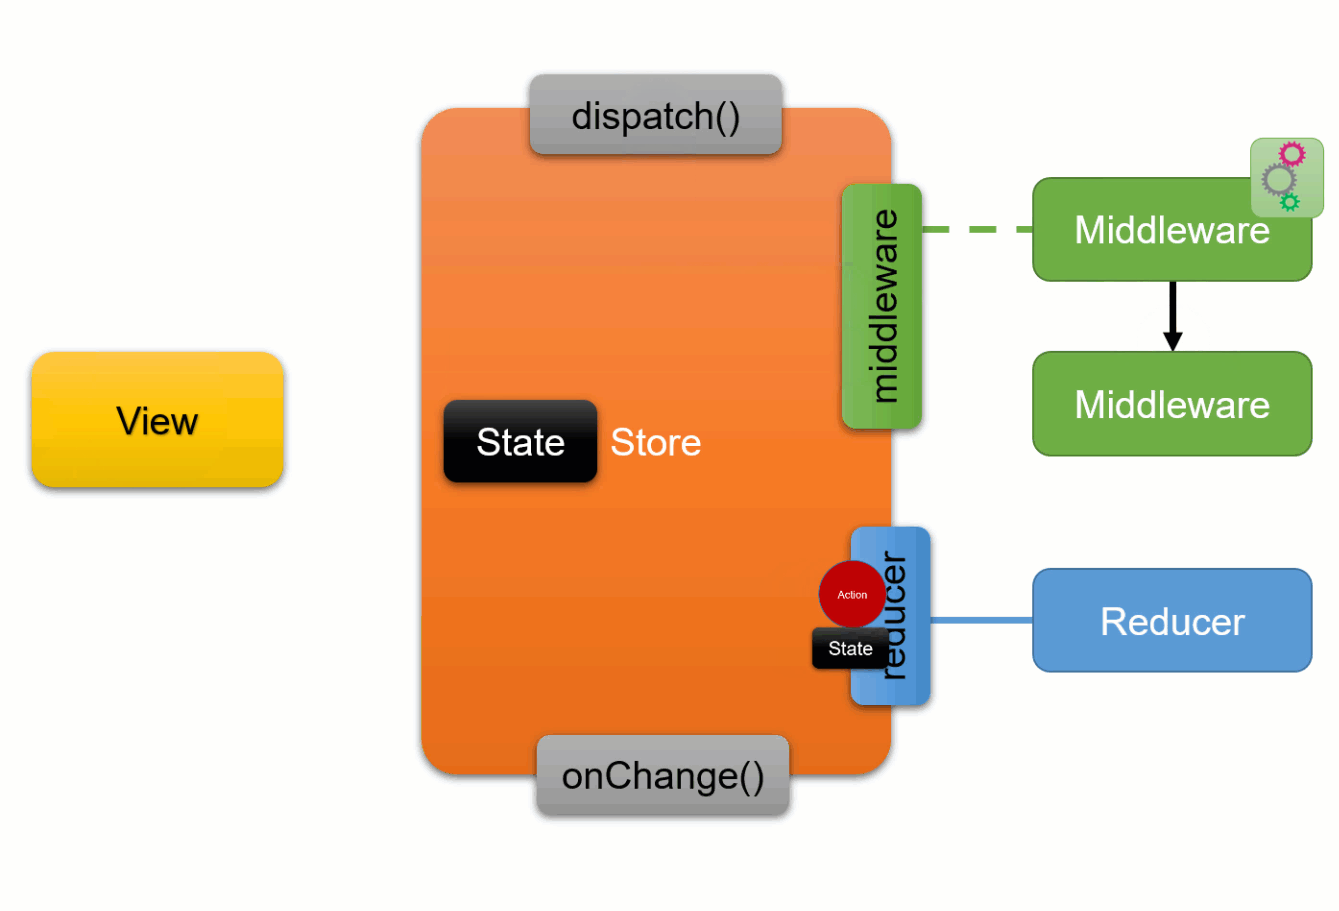
\includegraphics[width=\figureWidthModifier\linewidth]{img/stand-van-zaken/redux-working-detailed-3.png}
    \caption{De Action en de State worden doorgestuurd de Reducer \autocite{Boelens2019}}
    \label{fig:redux-working-detailed-3}
\end{figure}

\begin{figure}[H]
    \centering
    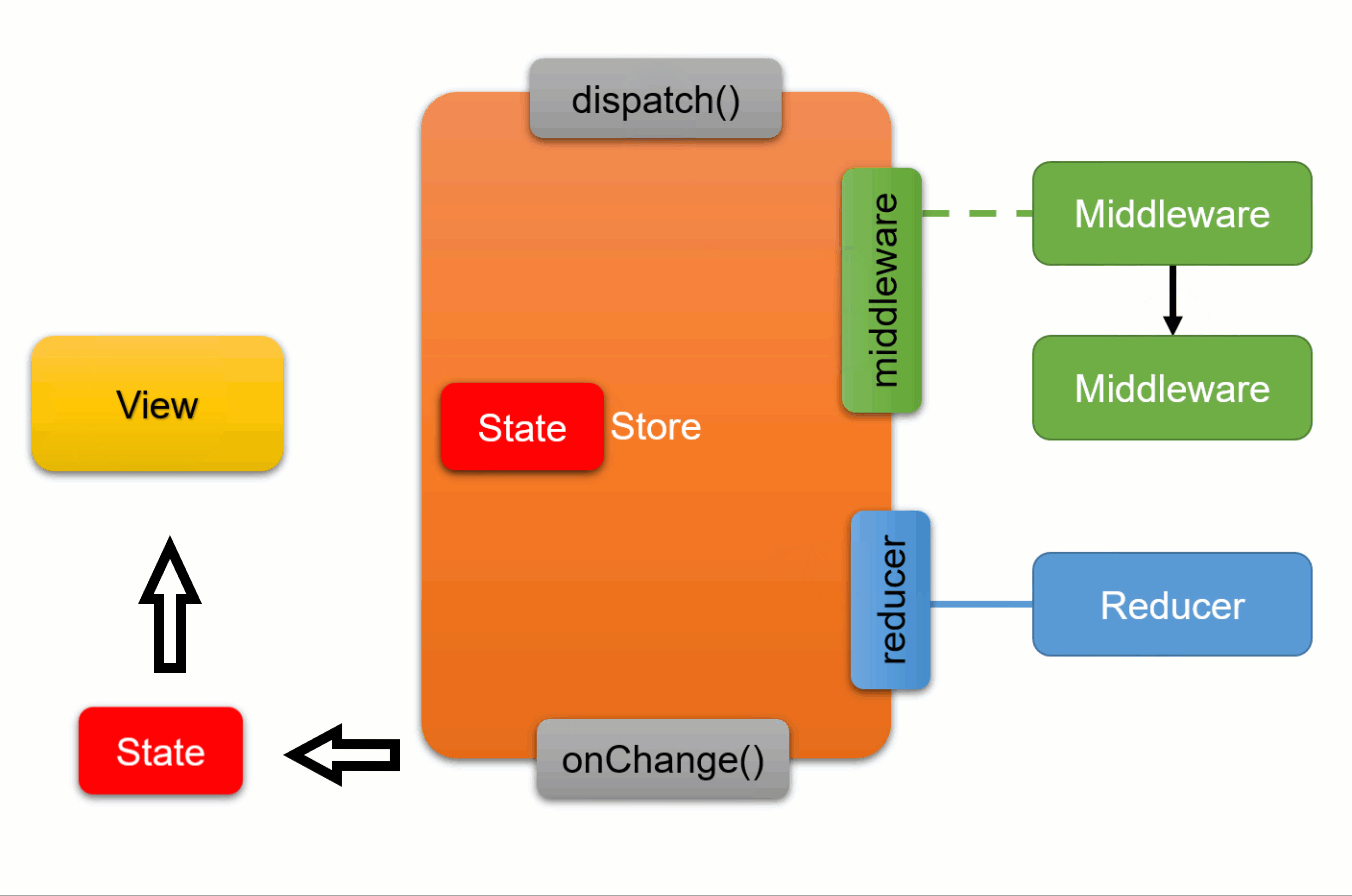
\includegraphics[width=\figureWidthModifier\linewidth]{img/stand-van-zaken/redux-working-detailed-4.png}
    \caption{De view wordt aangepast op basis van de nieuwe State \autocite{Boelens2019}}
    \label{fig:redux-working-detailed-4}
\end{figure}

In het \verb|flutter_redux| package zijn handige widgets beschikbaar. Zo zorgt de \verb|StoreProvider| widget ervoor dat de Redux Store wordt doorgegeven aan alle onderliggende widgets in de widget tree. De \verb|StoreBuilder| haalt de Store uit de \verb|StoreProvider| en geeft die door aan een widget builder function. Het nadeel bij de \verb|StoreBuilder| is dat de widget in de build functie telkens zal worden opnieuw opgebouwd wanneer de State wijzigt, dit kan leiden tot onnodige rerenders. De \verb|StoreConnector| biedt hiervoor de oplossing. De \verb|StoreConnector| haalt de Store uit de dichtstbijzijnde StoreProvider voorouder en zet de Store om in een ViewModel. Dit ViewModel zal alleen de waarde bevatten dat van belang is voor desbetreffende widget. Zo wordt een widget niet onnodig opgebouwd wanneer de Store wijzigt, maar alleen wanneer de waarde, gespecifieerd in de ViewModel, wijzigt. Bijvoorbeeld: de Redux Store bevat een counter waarde en een willekeurige tekst, de code voor de StoreConnecter wordt de volgende: 

\begin{minted}{dart}
new StoreConnector<int, CounterViewModel>(
    converter: (store) => CounterViewModel.from(store),
    builder: (context, counterViewModel) {
        return Text(counterViewModel.value);
    },
);
\end{minted}
Hier zal de Text widget alleen heropgebouwd worden wanneer de waardes die relevant zijn voor het CounterViewModel wijzigen.


\subsection{MobX}
\label{ch:mobx}
\subsection*{Principes}
MobX is opnieuw een library die bekend is bij ontwikkelaars. MobX is beschikbaar in Flutter via de package \verb|mobx| op pub.dev. MobX is een state management bibliotheek om de gegevens van de applicatie op een simpele manier te verbinden met de UI. Deze verbinding gebeurt volledig automatisch. De ontwikkelaar focust zich enkel op de data die in de UI getoond moet worden zonder zich zorgen te maken over het feit dat deze in sync moeten staan.

MobX maakt gebruikt van drie belangrijke concepten: \textbf{Observables}, \textbf{Actions} en \textbf{Reactions}.
\newline
De Observables bevatten de state van de applicatie. Een Observable kan een primitief datatype zijn tot een zelf geschreven klasse. Met de volgende lijn code wordt een Observable geïnstantieerd. \verb|final counter = Observable(0);|.

De Actions definiëren hoe de Observables gemuteerd moeten worden. Opnieuw is, zoals in Redux, een scheiding gemaakt zodat de waarden nooit direct aangepast kunnen worden.
Een voorbeeld van een Action:
\begin{minted}{dart}
final increment = Action((){
    counter.value++;
});    
\end{minted}

De Reactions voltooien de MobX-triade. De Reactions zijn de waarnemers van de Observables. Een Reaction houdt als het ware een Observable bij. Telkens wanneer een Observable wijzigt, wordt de Reaction verwittigd. Er zijn een paar verschillende vormen van een Reaction, maar deze geven allemaal een \verb|ReactionDisposer| terug. Deze \verb|ReactionDisposer| is een functie dat kan wordt opgeroepen om de reaction weg te verwijderen uit het geheugen. Een voorbeeld van de \verb|autorun| Reaction:
\begin{minted}{dart}
int counter = Observable(0);

final dispose = autorun((_) {
    print(counter);
});

counter = 1;

dispose();

// Prints:
// 0
// 1
\end{minted}

Deze drie principes zijn terug te vinden op figuur \ref{fig:mobx-principles}:

\begin{figure}[H]
    \centering
    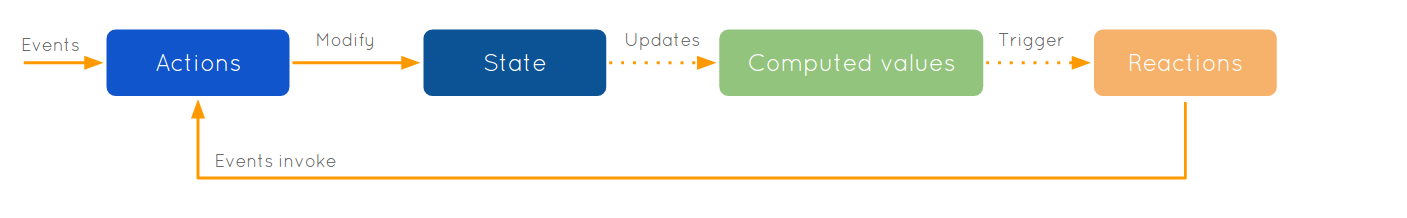
\includegraphics[width=\linewidth]{img/stand-van-zaken/mobx-principles.png}
    \caption{Flowchart van MobX \autocite{MobX2019}}
    \label{fig:mobx-principles}
\end{figure}

Een ander begrip dat terug komt in MobX is een Store. Dit is een klasse die de bijhorende Observables zal bevatten. Bijvoorbeeld een counter Store zal de waarde bijhouden van de counter inclusief een actie om deze te incrementeren.

De  \verb|flutter_mobx| package bevat tal van handige widgets zoals een Observer widget die automatisch wordt opgebouwd wanneer de waarde van een Observable wijzigt. 
Om de Store klasse leesbaar te houden wordt gebruikt gemaakt van \verb|mobx_codegen|. Deze package zorgt dat er geen boilerplate code geschreven moet worden. 
